\documentclass[11pt]{article} 
\usepackage[pdftex]{graphicx}
 
\title{CS350 QuickHull Project Report}
\author{Gregory Haynes and Eric O'Connell}
\date{December 1 2011}

\begin{document}

\maketitle

\section{Introduction}

In mathematics the convex hull of a set of points X is the minimum convex set containing X. In this paper we will describe an efficient method for computing the convex hull of a set. There are many practical applications of the problem of determining convex hulls which range from Image processing to static code analysis which make the discovery of efficient algorithms to compute convex hull a worthwhile subject.

\section{Algorithm Explanation}

The quickhull algorithm, given its name due to its similarity to the quicksort algorithm, is a fast method for determining the convex hull of a set of points. The algorithm has two phases. The first phase splits the set into an upper and lower portion using a chord between two points known to be on the convex hull (these two points are also added to the set of points on the hull). The next phase of the algorithm takes the chord and a set of points to one side of the chord. This phase recursiveley determines the farthest point from the chord, then adds this point to set set of convex hull points, and recursively computes the convex hull on the points outside the triangle formed by these three points. A more detailed description is provided in the Quickhull Psuedocode.

\subsection{Quickhull Pseudocode}

\textbf{TrianglePartition(P, A, B):}
\begin{verbatim}
If P is the empty set return the empty set
Let C be the farthest point from the line containing A and B
Let L be a subset of P where each element is left of the line A..C
Let R be a subset of P where each element is left of the line C..B
Let CH <- TrianglePartition(L, A, C) + {CH}
   + TrianglePartition(R, C, B)
Return CH
\end{verbatim}
\textbf{Quickhull(P):}
\begin{verbatim}
Let C be a chord from point C.a to C.b where 
   both C.a and C.b are points on the convex hull of P
Let U be a subset of P where each element in U is above C
Let L be a subset of P where each element in L is below C
Let CH <- {C.a} + TrianglePartition(P, C.a, C.b) + 
   {C.b} + TrianglePartition(P, C.b, C.a)
Return CH
\end{verbatim}

\subsection{Pivot Chord Selection}
The pivot chord selection in quickhull plays a major role in the efficiency of the algorithm, much like in its quicksort counterpart. For this project the chord was selected by finding the maximum and minimum values along the X axis. This could be easily modified to select a chord along the Y. More advanced chord selection techniques are beyond the scope of this project.

\section{Implementation}
Our quickhull algorithm was implemented using JavaScript. This language was chosen due to the ease with which results could be visually displayed using minimal HTML code. Aditionally, recent advancements in JavaScript interpreters allow for reasonably fast execution of the algorithm.

\subsection{Verification}
To verify the correctness of our quickhull implementation we developed a brute force convex hull algorithm and compared the outputs of these two algorithms. We compared the output of these two algorithms using 10,000 iterations of random point data with a uniform distribution. We also compared the algorithms using random points on circles and lines.

\subsubsection{Brute Force Psuedocode}
\begin{verbatim}
Let CH be an empty set
For each pair of points (A, B):
   If all points in P are below the vector A..B then add A, B to CH
Return CH
\end{verbatim}

\section{Analysis}

\subsection{Complexity}
The quickhull algorithm has a worst case running time of $O(n^2)$. This can be seen by constructing a recurrence relation for the worst case of TrianglePartition (see quickhull psuedocode). The worst case is when the triangle ABC does not contain any points (other than A, B, C). In this case, only one point is eliminated from the set of possible points. Additionally finding C requires O(n) time, thus the recurrence relation is:
\[ T(n) = T(n - 1) + T(n - 1) + O(n) \]
After expansion this recurrence releation solves to $O(n^2)$ complexity.
\\
\\
With an evenly spaced distribution we can expect the trangle ABC to encompass half of the points, which gives us the following recurrence relation
\[ T(n) = T(n / 2) + T(n / 2) + O(n) \]
Using the Master Theorem we can solve this recurrence relation as being $O(n log(n))$ complexity.

\subsection{Experimental Performance}
In order to determine the efficiency of the algorithm as implemented, we used the JavaScript console.profile API to measure successive runs of quickhull on increasingly-large sets of points. As a basis point of comparison, we also measured the running time of the brute-force function.

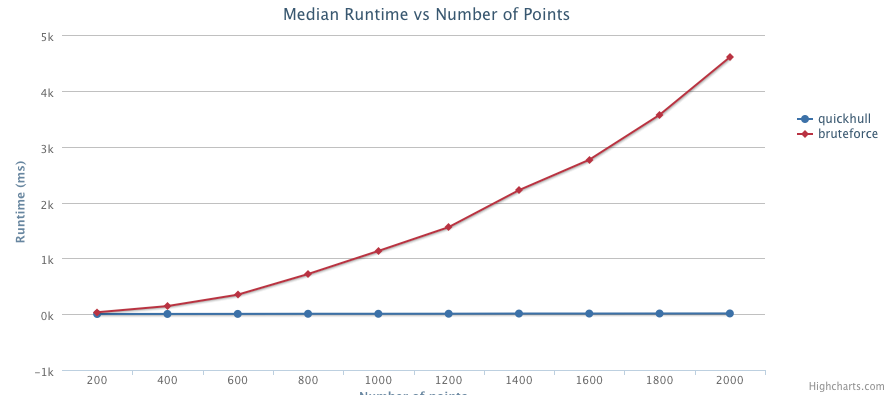
\includegraphics[scale=0.3]{quickhull - raphael-cloud.png} 
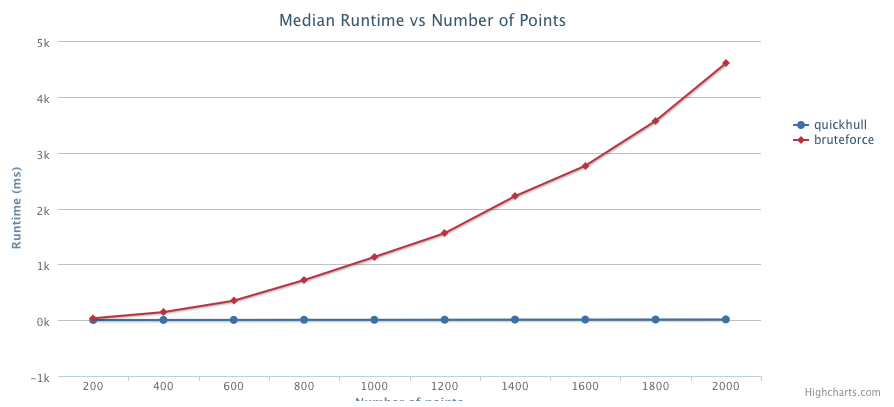
\includegraphics[scale=0.3]{quickhull - raphael-circle.png} 

\subsection{Other Convex Hull Algorithms}
Grahams scan is another popular convex hull algorithm which has a worst case running time of $O(nlog(n))$. This algorithm first performs a clockwise sorting of the points and then determines, in order, which points are on the convex hull.

\section{Summary}

\section{Citations}

\end{document}
